\section{The FPGA engine}
\label{sec:fpga}

The field is a better fit for an FPGA than for a GPU: the GPU has one
narrow carry-less unit per SM, while the FPGA is nothing but
carry-less multipliers, and $\sigma^k$ is wiring. A VHDL engine for
the AWS F2 (Xilinx VU47P) was designed, estimated before any board
time, and then measured.

\subsection{Estimate before the board}
\label{sec:fpga-estimate}

Before synthesis, the client's own straight-line multiplier was
mapped to LUT6s (about $5{,}563$ at 32 levels, known to be about $40\%$
high for ignoring dual-output packing) and calibrated against the
$3{,}071$ and $3{,}620$ LUTs that Bernstein et al.\ report for
$\mathrm{GF}(2^{113})$ and $\mathrm{GF}(2^{127})$
multipliers~\cite{bernstein2016fpga}, extrapolated to $3{,}781$ at
$m=131$. With multipliers at $79\%$ of a core and $5.33$ multipliers
per core, a core is $25.5$~KLUT at literature packing or $37.5$~KLUT
with the repository's unpacked circuit; $18\%$ shell overhead on
$1{,}303{,}680$ CLB LUTs at $70$--$80\%$ utilisation gives 29--34 or
20--23 cores at an estimated $250$--$350$~MHz. The estimate was
$5$--$12$~B iterations/s per VU47P, central $8$~B/s: slower per chip
than the $14.1$~B/s GPU, about level on cost per solve, and $2$--$5\times$
better per watt.\art{ecc2k130/FPGA-CEILING.md}

\subsection{Design}
\label{sec:fpga-design}

\paragraph{Multiplier.} \texttt{gf131\_mul} follows the Bernstein--Lange
route in hardware: \texttt{prep} converts each operand to the
polynomial basis (991 XOR2 per operand), a recursive Karatsuba
\texttt{gf2\_kmul} splits $131\to66\to33\to17$ bits into 27 leaf
products of $17\times17$, and \texttt{to\_onb} converts the
261-coefficient product back ($3{,}167$ XOR2). There is no reduction
step. At three levels the product is $7{,}803$ AND and $9{,}404$ XOR2,
$14{,}553$ XOR2 per multiply including conversions, against $17{,}161$
AND and $22{,}049$ XOR2 for schoolbook. Out of context in Vivado 2025.2
at a $4.0$~ns clock, three levels map to $4{,}855$ LUTs and $4{,}647$
FFs with $+2.68$~ns of slack.\art{hdl/ecc2k130/README.md}

A DSP leaf computes a $17$-bit $\mathrm{GF}(2)$ product as six
$25\times16$ integer products with coefficients spaced three bits
apart (split $9+8$ against $6+6+5$) so that no column count exceeds
six and nothing carries; the parities are XORed into place with 22
LUTs. Eleven of the 27 leaves go to DSPs, 66 DSP48E2 per multiplier,
which takes the multiplier to $4{,}004$ LUTs at a latency of 14 clocks
including a 261-FF copy register (11 clocks with LUT leaves). The
pblock holds $7{,}992$ DSPs, so 120 engines can take 11 DSP leaves and
128 engines ten.\art{hdl/ecc2k130/gf2_dsp_leaf.vhd}\art{hdl/ecc2k130/README.md}

\paragraph{Step and batch.} An unbatched step is ten multiplies:
$d=x+\sigma^j x$, $\lambda=(y+\sigma^j y)/d$ with the eight-multiply
Itoh--Tsujii inversion, $x_3=\lambda^2+\lambda+d$,
$y_3=\lambda(x+x_3)+x_3+y$. \texttt{ec2k\_batch\_pipe} shares one
inversion across $W$ walks through a product tree held in UltraRAM
(four URAM288 per engine): $W-1$ forward multiplies, 8 for the
inversion, $2(W-1)$ backward, $W$ for $\lambda$ and $W$ for $y_3$,
$5W+5$ per batch, $5+5/W$ per step: $5.31$ at $W=16$, $5.16$ at $W=32$,
$5.08$ at $W=64$. A batch is a chain of $2\log_2 W+10$ bursts, and
several batches are kept in flight to hide the multiplier latency.
Table~\ref{tab:fpga-sim} is the simulated rate.\art{hdl/ecc2k130/ec2k_batch_pipe.vhd}\art{hdl/ecc2k130/README.md}

\begin{table}[t]
\centering
\small
\caption{Simulated clocks per step of the batched step unit at
  multiplier latency 10, against the arithmetic bound $5+5/W$. The
  default geometry is $64\times8$ (512 walks per engine), which runs
  at $5.16$ clocks per step with either multiplier.}
\label{tab:fpga-sim}
\begin{tabular}{@{}rrrrr@{}}
\toprule
$W$ & batches in flight & 200 steps & $6{,}144$ steps & bound \\
\midrule
8 & 8 & 8.02 & 6.62 & 5.63 \\
16 & 4 & 9.86 & 8.38 & 5.31 \\
16 & 8 & 6.98 & 5.67 & 5.31 \\
16 & 16 & 6.46 & 5.34 & 5.31 \\
32 & 8 & 7.20 & 5.20 & 5.16 \\
\bottomrule
\end{tabular}
\end{table}

\paragraph{Walker and host port.} Walks live in a block-RAM FIFO of
$(\mathrm{id},\mathrm{steps},x,y,\mathrm{dp})$, 285 bits by 512, read
through a four-entry prefetch. Only the low 13 bits of the step count
travel with the walk; the high 19 sit in a LUTRAM table bumped once
every $8{,}192$ steps. A step whose $x$ has weight at most
\texttt{DP\_WEIGHT} is flagged, moves into a report register at the
FIFO head and is held until acknowledged, so no report is ever lost
and the \texttt{DROPPED} counter always reads zero. \texttt{ec2k\_axil}
is an AXI4-Lite slave in front of \texttt{NENG} walkers with a
credit-based register spine (about 870 FFs and 300 LUTs per engine),
introduced after the first flat 48-engine build placed at
$-2.5$~ns. The host program is a drop-in for the CUDA client under
the same worker script: it writes the same 32-byte records and
re-walks every report from its seed on the CPU.\art{hdl/ecc2k130/ec2k_walker.vhd}\art{hdl/ecc2k130/host/ecc2k130_fpga.cpp}

\paragraph{Verification.} The reference script imports the client's
field model and emits 256 multiplier vectors (including 0, the
all-ones 1, single basis elements and the extreme coordinates, each
also checked against an independent direct convolution), 200 steps
(twelve full batches of 16 plus a partial batch, so the flush path
runs every time) and 64 walks of random order-$\ell$ points on the
challenge curve. The batch testbench passes for every $W$ from 2 to
32 with 2 to 16 batches in flight; the walker testbench checks every
report's id, step count and point against the reference trajectory
(64 distinguished points from 797 steps in $19{,}194$
clocks).\art{hdl/ecc2k130/ecc2k_ref.py}\art{hdl/ecc2k130/vectors_ecc2k130.txt}

\subsection{Measured on \texttt{f2.6xlarge}}
\label{sec:fpga-measured}

\begin{table}[t]
\centering
\small
\caption{F2 images on one VU47P (\texttt{f2.6xlarge}). All runs had
  zero dropped reports; 32 or 64 sampled distinguished points per
  image were re-walked on the host against the client reference from
  the same seed and matched. The 128-engine image is the promoted
  AFI.}
\label{tab:fpga-images}
\begin{tabular}{@{}rrlrrr@{}}
\toprule
engines & MHz & geometry & routed WNS (ns) & M steps/s & clk/step \\
\midrule
48 & 333.3 & $16\times16$, tree in BRAM & $+0.022$ & $3{,}010.7$ & 5.31 \\
64 & 333.3 & same & $+0.040$ & $4{,}013.7$ & 5.32 \\
80 & 333.3 & 17 tiles/engine & $+0.027$ & $5{,}015.8$ & 5.32 \\
96 & 333.3 & same & $+0.002$ & $6{,}018.0$ & 5.32 \\
112 & 375 & $32\times8$, tree in URAM & $+0.049$ & $8{,}123$ & 5.17 \\
120 & 333.3 & $32\times8$, tree in URAM & $+0.063$ & $7{,}730$ & 5.17 \\
\textbf{128} & \textbf{333.3} & $32\times8$, tree in URAM, LUT multiplier & $+0.048$ & $\mathbf{8{,}249}$ & \textbf{5.17} \\
\bottomrule
\end{tabular}
\end{table}

Table~\ref{tab:fpga-images} is every image that was built, placed,
loaded and timed, and Figure~\ref{fig:fpga} draws it.\art{hdl/ecc2k130/aws/README.md}
The 48-engine run read back its geometry (48 engines of 512 walks,
weight 34, $333.3$~MHz), seeded $24{,}576$ walks over AXI-Lite in
$7.3$~s, held $3{,}010$~M steps/s from ten seconds on, and completed
$103$~G iterations in a 40~s run; simulation had predicted $5.29$
clocks per step against the measured $5.31$. The promoted 128-engine
image holds $8.25$~G steps/s. Linear scaling with engine count is the
prediction of a design that shares nothing between engines except the
host port, and the measured images sit on it. Builds that missed
timing (128 engines at 375~MHz, 112 at 400) and the 144-engine build
that failed block-RAM placement ($3{,}744$ RAMB18 sites needed against
$3{,}576$) are recorded alongside; the projection at $5.16$ clocks per
step is $8.8$~G at 136 engines and $9.3$~G at 144 or at 128 engines
and 375~MHz, neither yet routed.

\begin{figure}[t]
\centering
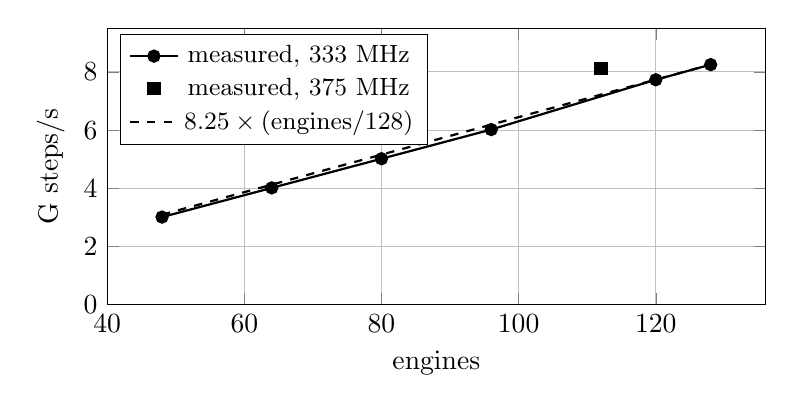
\begin{tikzpicture}
\begin{axis}[
  width=0.82\textwidth,
  height=0.42\textwidth,
  xlabel={engines},
  ylabel={G steps/s},
  xmin=40, xmax=136,
  ymin=0, ymax=9.5,
  grid=major,
  legend style={at={(0.02,0.98)},anchor=north west,font=\small},
]
\addplot[mark=*,thick] coordinates {
  (48,3.0107) (64,4.0137) (80,5.0158) (96,6.018) (120,7.73) (128,8.249)
};
\addlegendentry{measured, $333$~MHz}
\addplot[mark=square*,only marks,thick] coordinates { (112,8.123) };
\addlegendentry{measured, $375$~MHz}
\addplot[dashed,domain=48:128,thick] {0.06445*x};
\addlegendentry{$8.25\times(\mathrm{engines}/128)$}
\end{axis}
\end{tikzpicture}
\caption{ECC2K-130 FPGA engine on AWS F2. The 128-engine image at
  $333$~MHz is $8.25$~G steps/s; the pre-board estimate was
  $5$--$12$~G with a central $8$~G. The measurement landed on the
  central estimate and is a device number, not the estimate reprised.}
\label{fig:fpga}
\end{figure}

Per engine the current revision is $6{,}790$--$6{,}940$ LUTs, $9{,}371$
FFs, 12 RAMB36, 4 URAM and 66 DSPs; the 96-engine image used $62\%$ of
the LUTs and $81\%$ of the block RAM, and block RAM, not logic, is
what bounds the engine count on this part.\art{hdl/ecc2k130/README.md}

\subsection{F2 against the GPU}
\label{sec:fpga-vs-gpu}

At the prices observed on 2026-09-11, an F2 instance at $\$1.980$
on demand or $\$0.709$ spot against an RTX~PRO~6000 at $\$4.14$ and
$\$1.31$ per GPU-hour, the expected $2^{60.9}$ iterations cost about $72{,}400$
F2-hours at the measured $8.25$~G/s, roughly $\$51$k spot, against
$42{,}400$ GPU-hours and $\$56$k spot at the campaign's $14.11$~B/s
collection rate.\footnote{Derived here from the measured rate and the
prices recorded in \texttt{ecc2k130/FPGA-CEILING.md}; the note's own
table priced the hypothetical $8$~B/s image at $\$53$k spot.} The
two platforms are therefore level on cost per solve within the noise
of spot pricing, and the FPGA is about $2$--$5\times$ better per watt
on the note's estimated envelopes ($75$--$150$~W against a $600$~W
board). FPGA workers speak the same client contract as the GPUs and
write the same records, so a collision between an FPGA trail and a
GPU trail is an ordinary merge.
